% conclusion
%
% CONCLUSION: Limitations of the study, Questions for further research.
%
%----------------------------------------------------------------------------------------
%	PACKAGES AND OTHER DOCUMENT CONFIGURATIONS
%----------------------------------------------------------------------------------------
% none

\section{Conclusion}
\subsection{Model Validation}
The reliability of the chosen model, prediction rule, and prediction error rate from the training data is examined by now applying the prediction rule to the validation data set (i.e. the remaining 20\% of data). As I will show, the new prediction error rate is about the same as that for the model-building data set, and gives a reliable indication of the predictive ability of the fitted logistic regression model and the chosen prediction rule. If the new and unseen data had lead to a considerably higher prediction error rate, then the fitted logistic regression model and the chosen prediction rule would not predict new observations well. \par
In my Prostate Cancer logistics model, the fitted logistic regression function (Eqn. 7) based on the model-building data set:

\[
\hat{\pi}=[ 1+ exp(-2.6867 + 1.0577X_1 + 1.5502X_2)]^{-1}
\]

was used to calculate estimated probabilities \(\hat{\pi}_h\) for the validation data set. The chosen prediction rule (Eqn. 14):

\[
	\textrm{Predict 1 if } \hat{\pi}_h \geq 0.20\textrm{; predict 0 if } \hat{\pi}_h < 0.20
\]

was then applied to these estimated probabilities. The percent prediction error rates are summarized in Figure 16 and Table 3 below:

\begin{figure}[H]
	\centering
	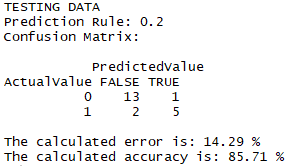
\includegraphics[scale=0.9]{confusion_matrix_final}
	\caption{Confusion Matrix - Validation Data}
\end{figure}

\begin{table}[H]
	\centering
	\begin{tabular}{ |c|c||c| }
 	\multicolumn{2}{c}{\underline{Disease Status}} \\
 	\hline
 	With High Grade Cancer&Without High Grade Cancer&Total\\
 	28.57\%&7.14\%&14.29\%\\
 	\hline
	\end{tabular}
 	\caption{Percent Prediction Error Rates - Validation Data}
\end{table}

Note that the total prediction error rate of 14.29\% is approximately equal to, or very similar to, the 15.79\% error rate based on the model-building data set. Therefore the latter is a reliable indicator of the predictive capability of the fitted logistic regression model and the chosen prediction rule.

\subsection{Final Remarks}
The interpretation for multiple logistic regression is that the estimated odds ratio for the predictor variable \(X_k\) assumes that all other predictor variables are held constant. In view of the fitted model (Eqn. 7) the estimated coefficients are: \(\beta_0 = -2.6867\), \(\beta_1 = 1.0577\), and \(\beta_2 = 1.5502\).
Therefore we can see, for instance, that the odds of a man being diagnosed with high grade prostate cancer increase by about 5.8\% for each additional score of PSA Level, for a given Cancer Volume. This means each unit increase of PSA Level increases the odds of said diagnosis by 5.8\%. Likewise, the odds of a man being diagnosed with high grade prostate cancer increase by  55.0\% for each unit increase in cancer volume. These calculated odds ratios suggest that Cancer Volume has a significantly larger association to the outcome, a diagnosis of high grade prostate cancer, than PSA Level. \par 


